%\documentclass{sig-alternate}
\documentclass{sig-alternate-05-2015}
\usepackage{graphicx}
\usepackage{pifont}
\usepackage{url}
\usepackage{code}
\usepackage{amsmath}
\usepackage{algpseudocode} 
\usepackage{algorithmicx}
\usepackage{algorithm}
\usepackage{xcolor}
%\usepackage{flushend}

\newcommand{\mycomment}[1]{}

\title{One Test Case to Rule Them All}
%\title{Normalizing and Generalizing Test Cases}

\numberofauthors{3}

\author{
\alignauthor
Alex Groce\\
       \affaddr{School of Electrical Engineering and Computer Science}\\
       \affaddr{Oregon State University}\\
%       \email{agroce@gmail.com}
% 2nd. author
\alignauthor
Josie Holmes\\
       \affaddr{Department of Geography}\\
       \affaddr{Pennsylvania State University}\\
%       \email{webmaster@marysville-ohio.com}
% 3rd. author
\alignauthor Kevin Kellar\\
       \affaddr{Crescent Valley High School}\\
%       \affaddr{1 Th{\o}rv{\"a}ld Circle}\\
%      \affaddr{Hekla, Iceland}\\
%      \email{larst@affiliation.org}
}

\mycomment{

\author{\IEEEauthorblockN{%
Alex Groce,\IEEEauthorrefmark{1}
Josie Holmes\IEEEauthorrefmark{2}
Kevin Kellar\IEEEauthorrefmark{3}
}

\IEEEauthorblockA{\IEEEauthorrefmark{1}%
School of Electrical Engineering and Computer Science\\
Oregon State University\\
\IEEEauthorrefmark{2}
Department of Geography\\
Pennsylvania State University
\IEEEauthorrefmark{3}
Crescent Valley High School
}


}
%\author{\IEEEauthorblockN{Alex Groce, Amin Alipour, Chaoqiang Zhang, Yang Chen, John Regehr}
%\IEEEauthorblockA{School of Electrical Engineering and Computer Science\\
%Oregon State University, Corvallis, OR\\
%Email: agroce@gmail.com, alipourm,zhangch@onid.oregonstate.edu}}
}

\mycomment{
\numberofauthors{1}
\author{
\alignauthor
Arpit Christi, Matthew Lyle Olson, Mohammad Amin Alipour, Alex Groce\\
\affaddr{School of Electrical Engineering and Computer Science}\\
\affaddr{Oregon State University}
\affaddr{Corvallis, OR USA}\\
%\affaddr{Corvallis, OR}\\
%\affaddr{USA}
}
}

\begin{document}

\maketitle 

\begin{abstract}
The difficulty of writing test harnesses is a major obstacle to the
adoption of automated testing and model checking.  Languages designed
for harness definition are usually tied to a particular tool and
unfamiliar to programmers; moreover, such languages can limit
expressiveness.  Writing a harness directly in the language of the
software under test (SUT) makes it hard to change testing algorithms,
offers no support for the common testing idioms, and tends to
produce repetitive, hard-to-read code.  This makes harness
generation a natural fit for the use of an unusual kind of domain-specific language (DSL). This paper defines a \emph{template
scripting} testing language, TSTL, and shows how it can be used to
produce succinct, readable definitions of state spaces.  The concepts
underlying TSTL are demonstrated in Python but are not tied to it.


\end{abstract}

\begin{CCSXML}
<ccs2012>
<concept>
<concept_id>10011007.10011074.10011099.10011102.10011103</concept_id>
<concept_desc>Software and its engineering~Software testing and debugging</concept_desc>
<concept_significance>500</concept_significance>
</concept>
</ccs2012>
\end{CCSXML}

\ccsdesc[500]{Software and its engineering~Software testing and debugging}

\printccsdesc

\keywords{test case reduction, semantic simplification, fuzzer taming,
  random testing, automated debugging}

\section{Introduction}

Software test automation encompasses two challenges: (1) automated
execution and determination of results for human-created tests, and
(2) truly automatic generation of tests.  Both are critical for effective,
efficient software testing, but only test generation offers the
potential to discover faults without human determination that a
particular execution scenario has the potential to behave incorrectly.
Automated generation of tests relies on the construction of \emph{test
  harnesses}.  A \emph{test harness} defines the set of valid tests
(and, usually, a set of correctness properties for those tests) for
the Software Under Test (SUT).  This paper presents a language and
tools applying insights from the world of explicit-state model
checking to the problem of producing test harnesses for automated
test generation, whether tests are produced by a exhaustive
state-space exploration as in model checking, or via less
systematic methods.

Building a test harness is a task that even experts in
model checking and automated testing often find painful
\cite{woda08,woda12}.  The difficulty of harness generation is one
reason for the limited adoption of automated testing and model
checking methods by the typical developer who writes unit tests.  This is
unfortunate, as even simple random testing can often uncover subtle
faults.

The ``natural'' way to write a test harness is as code in the language
of the SUT.  This is obviously how most unit
tests are written, as witnessed by the proliferation of tools like
JUnit \cite{JUnit} and its imitators (e.g., PyUnit, HUnit, etc.).  It
is also how many industrial-strength random testing systems are
written \cite{ICSEDiff,AMAI}.  A KLEE ``test harness'' \cite{KLEE} for
symbolic execution is written in C, with a few additional constructs
to indicate which values are symbolic.  This approach is common in
model checking as well: e.g., Java Pathfinder \cite{JPF,JPF2} can
easily be seen as offering a way to define a state space using Java
itself as the modeling language, and CBMC \cite{CBMC,CBMCp} performs a
similar function in C, using SAT/SMT-based bounded model checking
instead of explicit-state execution.  JPF in particular has shown how
writing a harness in the SUT's own language can make it easy to
perform ``apples to apples'' comparisons of various testing/model
checking strategies \cite{JPFRandTest}.


\begin{figure}[b]
{\scriptsize
\begin{code}
op = choice(operations);
val1 = choice(values);
val2 = choice(values);
if (op == op1 \&\& guard1) \{
    call1(val1);
\} else if (op == op2 \&\& guard2) \{
    call2(val1,val2);
\} else if (op == op3 \&\& guard3) \{
    call3(val1,val2);
...
\end{code}
}
\vspace{-0.15in}
\caption {A test harness in the SUT's language.}
\label{fig:badharness}
\end{figure}

Unfortunately, writing test harnesses this way is a highly repetitive
and error-prone programming task, with many conceptual ``code clones''
(e.g. Figure \ref{fig:badharness}). A user faces difficult choices in
constructing such a harness. For example, the example harness always assigns {\tt val2} even
though {\tt call1} only uses {\tt val1}, to avoid having to repeat the
choice code for calls 2 and 3.  The harness is almost certainly
sub-optimal for  random testing, where the lack of any
memory for previously chosen values can make it hard to exercise code
behaviors that rely on providing the same arguments to multiple method
calls (e.g., {\tt insert} and {\tt delete} for container classes).
The construction of a harness becomes even more complex in realistic
cases, where the tested behaviors involve building up complex types as
inputs to method calls, rather than simple integer choices. For
example, consider the problem of testing a complex Python library.  Figure
\ref{fig:MakeFeatureLayer} shows a portion of the Python documentation
for one function in the ArcPy \cite{ArcPy} site
package for Geographic Information Systems (GIS) automation.  Rather than taking a single integer, this
function call requires complex inputs --- a feature class or
layer, an SQL expression, and other complex types that we can assume
are also difficult to construct.  A harness testing a typical
real-world library must manage the creation of values of many such complex types.
Moreover, because building up function inputs is itself complicated
and requires complex method calls, these values cannot simply be produced on each iteration, but must be
stored and selected for use in future calls.
The code quickly becomes hard to read, hard to maintain, and hard to
debug.  In some cases \cite{AMAI} the code for a sophisticated test
harness approaches the SUT in complexity and even size!  The code's
structure also tends to lock in many choices that would ideally be configurable.

\begin{figure}[t]
{\scriptsize
\begin{code}
MakeFeatureLayer\_management(in\_features, out\_layer, {where\_clause}, {workspace}, {field\_info})
   
   Creates a feature layer from an input feature class or layer file. The layer
   that is created by the tool is temporary and will not persist after the session
   ends unless the layer is saved to disk or the map document is saved.
    
INPUTS:
 in\_features (Feature Layer):
   The input feature class or layer from which to make the new layer. Complex
   feature classes, such as annotation and dimensions, are not valid inputs to this tool.
 where\_clause \{SQL Expression\}:
   An SQL expression used to select a subset of features. For more information on
   SQL syntax see the help topic SQL reference for query expressions used in ArcGIS.
...
\end{code}
}
\caption{Documentation for a function in Esri's ArcPy site package.}
\label{fig:MakeFeatureLayer}
\end{figure}

One of the most important of these locked-in choices is the  test generation
method.  Writing a harness by hand usually makes it hard to try out
new strategies.   Writing novel testing strategies in even such
an extensible platform as Java Pathfinder is hardly a task for the
non-expert.
The harness in Figure \ref{fig:badharness} may support random testing and
some form of model checking, if it is written in Java and can use JPF
or a library for adaptation-based testing \cite{ISSRE12}. Such a
harness will likely be completely inflexible as to generation method if written in Python, C,
or another language without that level of tool support.

What the user really wants is to simply provide a concise version of the information in
Figure \ref{fig:MakeFeatureLayer}, some configuration details (e.g., how many
feature classes to keep track of at once), and then try different test
generation methods.  While some automated testing tools for Java \cite{FA11,Pacheco}
can automatically extract
method signatures from source code and produces tests,  
using such a tool locks a user into one test generation method.
Completely automatic extraction also often fails to handle
the subtle details of harness construction, such as defining guards
for some operations, or temporal constraints between API calls that
are not detectable by simple exception behavior.  Understanding
problems with automatic extraction can be hard with large libraries,
since the extraction tends to either produce internal data structures
only or produces a huge, impenetrable mass of code. The user \emph{wants} a
declarative harness, but often \emph{needs} to program critical details of a
harness, and build understanding of the system by performing harness development in
small, incremental steps.

\subsection{Contributions}

In this paper we describe a complete, Domain Specific Language (DSL)-based approach that combines
a simple means to produce a declarative harness with the full power of
a complete programming language.  TSTL (the Template Scripting Testing
Language) compiles a declarative description of system state and
actions into a library in the language of the System Under Test
(SUT).  This library allows the creation of objects providing an API
for testing the SUT, including support for state comparison,
abstraction, backtracking, automatic test case reduction, code coverage, and support
for sophisticated regression testing.

Using an ongoing case study,
we show how to apply TSTL and its tool suite to a large, real-world software
library used in critical applications.  The test effort has been driven and directed not by a
software testing researcher (as is the usual case), but by a domain
expert in the Geographic Information Systems (GIS) SUT.  In the
course of this effort, multiple faults and undocumented restrictions of the library
under test have been discovered, and the TSTL language and tool suite have
been transformed from a research prototype into a complete system for
software testing.

This paper presents the most complete presentation of the TSTL
language and tools, and we hope that it satisfies three critical goals:

\begin{itemize}
\item First, would-be users wanting to take advantage of automated
  test generation should be able to base their own testing
  efforts using TSTL on the example code in this paper (and that available
  in the TSTL github repository \cite{tstl}).
  This paper thus completely describes the concepts behind TSTL, the
  semantics of the language, and the tools available in TSTL.
  Previous papers on TSTL \cite{NFM15,ISSTA15} reported a much less full-featured version of the
  language using a difficult-to-read syntax.

\item Second, researchers should be able to use the information in this paper to
  extend existing TSTL tools or build their own tools to explore novel
  test generation strategies, automated debugging methods, and other
  research prototypes.  TSTL enables easy comparison of
  methods in a framework reducing the burden of implementation
  and avoiding irrelevant differences in performance due to underlying
  infrastructure.  The growing set of SUTs
  included in the TSTL distribution, which includes large and widely
  used Python libraries, can provide benchmarks for
  experimental efforts.  

\item Finally, unlike previous publications on TSTL, this paper
  emphasizes the fact that TSTL, unlike other testing DSLs or tools,
  at heart transforms a definition of valid tests (and properties) for
  a System Under Test into a \emph{programming language interface} for testing
  that system.  Tests in TSTL are not inaccessible entities internal to
  a tool,
  or only represented as unit tests (i.e., programs) that cannot be
  easily manipulated and analyzed, but first-class objects in the
  language of the System Under Test.  To our knowledge, this approach
  to testing has not been previously explored, and it was not
  emphasized (or even clearly presented) in earlier publications on TSTL.
\end{itemize}


The organization of this paper is as follows.  In Section
\ref{sec:dsltest} we present the basic idea of a DSL for testing, and
distinguish TSTL from other testing DSLs.  Section \ref{sec:arcpy} 
provides background on the ArcPy GIS case study used throughout the
paper.  Section \ref{sec:lang} provides a full description, with
examples, of the core TSTL language and semantics.  Section
\ref{sec:tools} describes the tools included with TSTL, and
Section \ref{sec:build} describes how researchers and developers can
build their own TSTL-based testing tools to support additional
testing, debugging, or regression strategies.  Section
\ref{sec:langext} introduces the novel TSTL concept of making testing
a first-class activity in a programming language, similar to how other
libraries make GIS (ArcPy), scientific computing (NumPy \cite{NumPy},
SciPy \cite{SciPy}) or bioinformatics
(QIIME \cite{QIIME}, Biopython \cite{biopython}, scikit-bio \cite{scikitbio}) activities simple to use in either a scripted or
interactive manner.  Faults discovered
using TSTL, in ArcPy and other systems, are described briefly in Section
\ref{sec:bugs}.  We survey the most closely related work in Section
\ref{sec:related}, and summarize our conclusions in Section \ref{sec:conclusion}.

\section{Domain Specific Languages for Testing}
\label{sec:dsltest}

The nature of test harness construction suggests the use of a
\emph{domain-specific language} (DSL) for testing \cite{ISOLA12}.  DSLs
\cite{Fow10} provide abstractions and notations to support a
particular programming domain. The use of DSLs is a formalization of
the long-standing approach of using ``little languages,'' as advocated by Jon Bentley in a
Programming Pearls column \cite{LitLang} and exemplified in such system
designs as UNIX.  DSLs typically come in two forms: \emph{external}
and \emph{internal}.  An external DSL is a stand-alone language, with
its own syntax.  An internal DSL, also known as a domain-specific
embedded language (DSEL), is hosted in a full-featured programming
language, restricting it to the syntax (and semantics) of that
language.  Many attempts to define harnesses can be seen as internal
DSLs \cite{UDITA,ISSRE12,JPF2,CBMCp,KLEE}.  Neither of these choices
is quite right for test harnesses.  Simply adding operations for
nondeterministic choice still leaves most of
the tedious work of harness definition to the user, and makes changing
testing approaches difficult.  With an external DSL, the user
must learn a new language, and the easier it is to learn, the less
likely it is to support the full range of features needed.

A novel approach is taken in recent versions of the SPIN model checker
\cite{SPIN}.  Version 4.0 of SPIN \cite{ModelDriven} exploited the
fact that SPIN works by producing a C program from a PROMELA model
to allow users to include calls to the C language in their PROMELA models.  The
ability to directly call C code makes it much easier to model check
large, complex C programs \cite{AMAI,ModelCode}.  C serves as a
``DSEL'' for SPIN, except that, rather than having a domain-specific
language inside a general-purpose one, here the domain-specific
language hosts a general-purpose language.  A similar embedding is
used in {\tt where} clauses of the LogScope language for testing Mars
Science Laboratory software \cite{scriptstospecs}.  We adopt this
approach for our own language and embed the general-purpose language (for expressiveness) in a
DSL (for concision and ease-of-use).

The most significant difference between TSTL and other DSLs for
testing and verification, including SPIN, is that most such systems
are primarily intended to be used as stand-alone tools.  Whether model
checkers \cite{SPIN,JPF2}, model-based testing tools \cite{Taxonomy},
or random testing tools \cite{Pacheco}, these systems are primarily
designed as ``things to \emph{run on} the system under test.''  TSTL
can operate in this manner, but at heart it transforms a definition of
valid tests into a library for creating, executing, manipulating, and
analyzing test cases.  An experienced TSTL user can interact with TSTL
at an interactive command prompt in the language of the SUT, creating,
saving, and modifying tests on-the-fly.  TSTL tools are simply
scripted formalizations of this mode of use, automating repetitive
tasks.  Such an approach is not possible with any other tool of which we
are aware.  Many tasks that are constrained to the functionality provided
by  tools included in other systems (e.g., replay of regression tests) in
TSTL are simplified and made flexible by this approach.

\subsection{TSTL: The Template Scripting Testing Language}

TSTL is based on understanding a test harness as a declaration
  of the possible actions the SUT can take, where these actions are
defined in the language of the SUT itself, with the full power
of the programming language to define guards, perform
pre-processing, and implement oracles.  Our particular approach is
based on what we call \emph{template scripting}.

The \emph{template} part of the name captures the fact that our method
proceeds by processing a harness definition file to output code that
enables testing, much  as SPIN processes PROMELA/C.  The harness
description file consists of fragments of code in the SUT's language
that are expanded, via the TSTL compiler, into a class that allows
an independently written test generation or manipulation tool to
generate, execute, or replay tests, without knowing
any details of the SUT.
A TSTL harness defines a \emph{template} for action definition, and
the compiler 
instantiates the template exhaustively.  The \emph{scripting} aspect indicates
TSTL is designed to be very lightweight and as easy for
users to pick up as a popular scripting language.  TSTL
works best when the SUT language is very
concise, like most scripting languages, making ``one-liners'' of action
definition possible; our initial implementation \cite{tstl} is therefore for
Python\footnote{We also have released a beta version of TSTL for Java \cite{TSTLJava}, to show
 that testing code in non-scripting languages is also possible.}.

\begin{figure}
{\scriptsize
\begin{code}
@from arcpy import *
\vspace{0.1in}
pools:
  <fc> 3 CONST             \# A feature class contains only lines, points, or polygons
  <newlayer> 3 CONST
  <op> 2 CONST 
  <val> 2 CONST
  <whereclause> 2 CONST    \# SQL clause to limit objects in new layers
  <fieldname> 2 CONST      \# Extracted from the shape files
  <fieldlist> 2
\vspace{0.1in}
actions:
\vspace{0.1in}
<fc> := <["d1.shp", "d2.shp", "d3.shp"]>  \# Just shapefiles for this example
<newlayer> := <["newl1", "newl2", "newl3"]>
\vspace{0.05in}
\{IOError\} <fieldlist> := ListFields(<fc>) \# Extract fields from a feature class
len(<fieldlist,1>) >= 1 -> <fieldname> := <fieldlist> [0].name 
<fieldlist> = <fieldlist> [1:] \# Skip to next field
\vspace{0.05in}
<op> := <[">", "<", "<=", ">=", "=", "!="]>
<val> := <1..10>
<val> = <val> * 10
<val> = <val> + 1

<whereclause> := '"' + <fieldname> + '" ' + <op> + str(<val>)
<whereclause> = <whereclause> + ' AND ' + <whereclause>
<whereclause> = <whereclause> + ' OR ' +  <whereclause>
<whereclause> = 'NOT' + <whereclause>

\{ExecuteError\} MakeFeatureLayer\_management(<fc>,<newlayer>)

\{ExecuteError\} MakeFeatureLayer\_management(<fc>,<newlayer>,where\_clause=<whereclause>)
\end{code}
}
\caption{A small TSTL file to test one ArcPy function.}
\label{fig:makefeaturelayer}
\end{figure}

\begin{figure}
{\scriptsize
\begin{code}
import sut, random, time
rgen = random.Random()
sut = sut.sut()
NUM\_TESTS = 1000
TEST\_LENGTH = 200 
for t in xrange(0,NUM\_TESTS):
   sut.restart()
   for s in xrange(0,TEST\_LENGTH): 
       action = sut.randomEnabled(rgen)
       r = sut.safely(action)
       if len(sut.newBranches()) > 0:
          print time.time(),'NEW BRANCHES:', sut.newBranches()
       if (not r) or (not sut.check()):
          pred = sut.failsCheck if r else sut.fails
          print 'TEST FAILED:', sut.error() 
          R = sut.reduce(sut.test(), pred)
          N = sut.normalize(R, pred) 
          sut.generalize(N,pred)
\end{code}
}
\caption{A simple random tester using the interface provided by TSTL.}
\label{fig:rt}
\end{figure}

Figure \ref{fig:makefeaturelayer} shows a simple TSTL harness for the
function documented in Figure \ref{fig:MakeFeatureLayer}.  Even this
short harness supports constructing SQL where clauses of arbitrary
length and selecting field names based on data files.  Figure
\ref{fig:rt} shows a simple pure random test generator that can test
any SUT (including this one) with a TSTL-defined harness.  This
harness, in 20 lines of code, not only provides automated test
generation, but continuous reporting of incremental branch coverage,
delta-debugging \cite{DD} for reduction of failing tests, and
additional TSTL-specific post-processing that further reduces the size
and complexity of test cases for debugging.  The brevity of the test
generator, no matter how complex the SUT, is made possible by the
common functionality of all TSTL-generated testing interfaces.  The
TSTL compiler produces a Python (or other target language) class that allows a test generation or manipulation
tool to view a testing problem as exploration of a (possibly infinite)
graph of states.  Transitions in the graph are the available test actions, executed in the underlying language, and are guarded by both TSTL
restrictions on the semantics of valid tests and user-defined guards
on system behavior.  States include both the (possibly unknown) state
of the SUT and the TSTL state, including pools of values to be used in actions.

In this simple example, the only ``oracle'' is the implicit property
that the system should neither crash nor raise an unexpected
exception.  For testing many systems, this is sufficient: we have
discovered real bugs in many Python libraries with only this level of
checking, similar to most of what a tool such as Randoop
\cite{Pacheco} or JCrasher \cite{CsallnerS04} checks.  TSTL also
checks arbitrary assertions/invariants defined in the language of the
SUT, supporting traditional property-based testing
\cite{ClaessenH00,hypothesis} (described in Section \ref{sec:property}).  Finally, TSTL includes sophisticated
support for differential testing \cite{Differential,ICSEDiff}, where a
system is tested with respect to the behavior of a reference library.
TSTL makes it easy to wrap a reference system to account for expected
differences, and supports partial reference testing (see Section \ref{sec:differential}).

\section{Motivating Case Study: Esri ArcPy}
\label{sec:arcpy}

Esri is the single largest GIS software vendor, with about 40\% of
global market share.  Esri's ArcGIS tools are extremely widely used
for GIS analysis, in government, scientific research, commercial
enterprises, and education.  Automation of complex GIS analysis and
data management is essential, and Esri has long provided tools for
programming their GIS software tools.  The newest such method,
introduced in ArcGIS 10.0, is a Python site-package, ArcPy
\cite{ArcPy}.  ArcPy is a complex library, with dozens of classes and
hundreds of functions distributed over a variety of of toolboxes.
Most of the code executed in carrying out ArcPy functions is the code
for the ArcGIS engine itself.  This source code, written in C++
(amounting to millions of lines), is
not available.  The source code for the latest version (10.3) of the
Python site-package alone, however, which interfaces with the ArcGIS
engine, is over 50,000 lines of code.  This is a very large system
(especially given the compactness of Python code), comparable in size
to the largest software systems previously tested using automated test
generation, such as core Java and Apache libraries
\cite{FA11,Pacheco}.

In order to improve the reliability of ArcPy, we are developing a
framework for automated testing of ArcPy itself, as well as libraries
based on ArcPy.  The TSTL harness for ArcPy is already more than six times as
large as the next-largest such definition previously implemented in
TSTL, even though the harness so far only includes a small portion of ArcPy
API (Application Program Interface) calls. The first stage of testing has resulted in discovery of
multiple faults in ArcPy/ArcGIS, and has required modifications to the
TSTL language and, especially, to the tool chain supporting test replay,
debugging, and test case understanding.

%One of the contributions of this paper is a more in-depth discussion
%of the problems, challenges, and tool utility aspects of testing
%software than is typical in most research papers in the field.  Such
%papers are (understandably) typically focused on novel algorithms or
%empirical evaluations of known methods, rather than the practical aspects of finding
%and understanding faults in a real-world software system.


%\subsection{Automated Testing for the Rest of the World}

Previous work on automated test generation for APIs has been largely carried
out by software testing researchers only, or (at most) by software
testing researchers working with individuals who are primarily
software developers.  This paper describes TSTL in the context of a
testing effort largely directed (and coded) by the first author, who is not a
software developer by profession or education, but a GIS analyst.
The problem of end-user testing
\cite{burnettEUSE,Silos,rothermelTOSEM} is long-standing.  Previous
work in the field has often focused on
non-traditional programming: e.g. spreadsheets
\cite{rothermelTOSEM}, visual languages, or machine-learning systems
\cite{OnlyOracle}.  TSTL is partly designed to allow a user who is
familiar with a software library but not expert in software testing
techniques to test a traditional software API library.  In one sense,
this is a less difficult scenario than spreadsheets
or visual forms, in that the testing is directed by an individual used
to writing and thinking about code.  The concepts in
automated software testing are most easily understood by those
who are also familiar with a conventional
programming language.  On the other hand, ArcPy is
not a small user-developed program but a large, complex system.
ArcPy was also not written by the end-user, or by any of the authors
of this paper, nor have the authors received any assistance in the
effort from Esri.

Automated testing systems more advanced than a simple hand-written
loop generating a few random inputs to a handful of functions, or more
complicated to use than a fully push-button system are often
considered too difficult for practical use even by software developers
or software QA staff \cite{ISSRE12}. Even ``push-button'' tools for
automated testing are sometimes difficult for expert users to install,
apply, and configure \cite{AMAI,CFV08,ISSRE12}.  TSTL aims to be
relatively easy to use for anyone familiar with basic Python
development.  By avoiding the use of a toy problem and presenting TSTL
in the context of a more typical real-world system (vs. e.g., a simple
container class), we hope to make it easier to apply to other
real-world systems.
%One goal of this work
%has been to mature the TSTL language and tool chain so Python
%programmers from all backgrounds can easily apply it to their
%automated testing problems, with tools approximately as easy to use as
%other Python developer tools.

%The second major contribution of this paper is therefore a presentation of an
%approach to automated testing that has been chosen by a GIS analyst, not a
%software developer or testing researcher.  Moreover, we present this
%paper as a proof-of-concept that modern automated testing, even in a
%highly interactive, non-push-button form, can be used by a motivated
%domain expert, with the support of  a domain-specific language
%\cite{Fow10} and a set of tools for generating, analyzing, and replaying tests.




\section{Formal Definitions}

%\subsection{A Brief Introduction to TSTL}

\begin{figure}[t]
{\scriptsize
\begin{code}
@import avl
\vspace{0.02in}
pool: <int> 4 CONST
pool: <avl> 3
\vspace{0.02in}
property: <avl>.check\_balanced()
\vspace{0.02in}
<int> := <[1..20]>
<avl> := avl.AVLTree()
\vspace{0.02in}
<avl>.insert(<int>)
<avl>.delete(<int>)
<avl>.find(<int>)
<avl>.inorder()
\end{code}
}
\caption{Part of TSTL harness for AVL trees.}
\label{fig:example}
\end{figure}

\mycomment{
\begin{figure}
{\scriptsize
\begin{code}
avl1 = avl.AVLTree()  
int3 = 10  
int1 = 11  
avl1.insert(int1) 
int1 = 1  
avl1.insert(int3) 
avl1.insert(int1) 
int3 = 9  
avl1.insert(int3) 
int2 = 11  
avl1.delete(int2) 
\end{code}
}
\caption{An example TSTL-produced test}
\label{fig:avlrun}
\end{figure}
}

TSTL \cite{NFM15,ISSTA15,tstlsttt} is a language for defining the structure of
tests (usually API-call sequences, but also grammar-based tests), and a set of tools for use in generating,
manipulating, and understanding those tests.  Figure
\ref{fig:example} shows a simplified portion of a TSTL definition
(called a harness \cite{WODA08,WODACommon}) of
tests for an AVL tree class, in the latest syntax for TSTL.
%TSTL provides features not shown in this small example,
%including differential testing, customizable logging, support for
%complex guards, and use of pre- and post- values.  
Given a harness
like the one in Figure \ref{fig:example}, TSTL compiles it into a
class file defining an interface for testing that provides features
such as querying the set of available testing actions, restarting a
test, replaying a test, collecting code coverage data, and so forth.
The TSTL release \cite{tstl} provides testing tools that use the
interface for testing and debugging.

The key point for our purposes is merely that a TSTL test harness
defines a set of \emph{pools} whose instances hold values produced and used
during testing \cite{AndrewsTR} (a common approach to defining
API-testing sequences) and a \emph{finite} set of actions that are possible during
testing, typically API calls and assignments to pool instances.  In this
example, there are two pools, one named {\tt int} and one named {\tt
  avl}.  There are four instances of the {\tt int} pool, which means
that a test in progress can store up to 4 {\tt int}s at one time (in
variables named {\tt int0}, {\tt int1}, {\tt int2}, and {\tt int3}), and three
instances of the {\tt avl} pool.  The actions defined are: setting
the value of an {\tt int} to any integer in the range 1-20
inclusive, setting the value of an {\tt avl} to a newly
constructed AVL tree, and calling {\tt insert}, {\tt
  delete}, {\tt find} and {\tt inorder} with chosen pool instances.  Figure
\ref{threetests} in the introduction shows three
valid tests produced by running a random test generator on
the TSTL-compiled interface produced by this definition.  TSTL handles
ensuring that tests are well-formed. No pool instance
(such as {\tt avl1}) can appear in an action until it has been assigned
a value.  No pool instance that has been assigned a value can be
assigned a different value until it has been used in an action, to
avoid degenerate sequences such as {\tt int3 = 10} followed by {\tt
  int3 = 4}.  Each action in a test is called a ``step'' --- the
first step of the first test in Figure \ref{threetests} is storing a new AVL tree in {\tt
  avl0}, for example.  A test is just an ordered sequence of
actions, which is equivalent to a set of numbered steps.  Because our
normalization is defined in terms of actions, steps, and pools, it is
language agnostic.

The definition of pools and actions in TSTL defines a \emph{total
  order} on all actions.  First, actions are ordered by their position
in the harness definition file.  All {\tt insert} actions therefore precede
all {\tt delete} actions, and all {\tt delete} actions precede {\tt
  find} actions.  One line of TSTL typically defines more than one action. For
example, the line {\tt <avl>.insert(<int>)} defines 12 actions, one
for each choice of {\tt avl} and {\tt int} pool instance, e.g.
{\tt avl0.insert(int0)}, {\tt avl1.insert(int0)}, and {\tt
  avl0.insert(int1)}.  These are
ordered lexically, with the first pool instance appearing in the text taking
precedence.  Value ranges, such as in the {\tt int} initialization, are also
ordered in the natural way, with lower values first.  Given this total
order, each action can be assigned a unique index, from 0 up to 1 less
than the total number of actions. Initially, this kind of ordering (and
numbering) for each action was intended to allow for a kind of
G\"odel-numbering of tests, for use in proofs about
properties of test-generation algorithms
\cite{AndrewsTR}.

The ordering of actions also allows us to concisely define a
practical method for normalizing tests, by
simple syntactic means, by considering an action ``simpler'' than another
action if it has a lower index.  One intuitive concern with normalization
based on action ordering is that a user may not place actions
in a ``good'' order.  What if normalization
rewrites actions into ``more complex'' actions?
The exact ordering usually \emph{does not matter}, it only
matters that there exists \emph{some ordering} to guide normalization
and generalization.  Actions will only be replaced or swapped if,
causally, the predicate (failure) is \emph{indifferent} to the choice.  The
normal form's \emph{existence} matters much more than the precise contents, in
the context of that semantic restriction.  In cases where there is a
clear notion of simplicity (e.g., more vs. fewer optional parameters
to a call, fewer array dimensions), simplest-first is often
also most natural in TSTL.

\subsection{Normalization}

A test normalization algorithm has a simple goal:  we ideally aim to
produce a function $f : t \rightarrow t$ (a function that takes a test
and returns a test) such that: (1) if $t$ fails, $f(t)$ fails\footnote{Normalization can
    be generalized to apply to any predicate over tests, not just
    failure \cite{icst2014}; a passing test can be normalized, though
    without some more interesting predicate, such as preservation of
    coverage, this is not clearly useful.}; (2) if $t_1$ and $t_2$ fail
  due to the same fault, $f(t_1) = f(t_2)$; (3) if $t_1$ and $t_2$ fail due to different faults, $f(t_1) \not=
  f(t_2)$.

\begin{comment}
\begin{enumerate}
\item If $t$ fails, $f(t)$ fails\footnote{Normalization can
    be generalized to apply to any predicate over tests, not just
    failure \cite{icst2014}.}.
\item If $t_1$ and $t_2$ fail due to the same fault, $f(t_1) = f(t_2)$.
\item If $t_1$ and $t_2$ fail due to different faults, $f(t_1) \not=
  f(t_2)$.
\end{enumerate}
\end{comment}

Such a function would define a true \emph{canonical form} for tests, where each underlying fault is uniquely represented by a single
test.  In general, it seems clear that defining such a function
$f$ is (at least) as difficult as automatic fault localization and
repair, and likely undecidable.  Therefore, we aim at approximating the
goal, by providing a set of simple transformations such that: (1) $f$
changes many tests to the same test, (2) $f$ has low probability of
changing two tests failing for different reasons into the same test,
and (3) $f$ is not unreasonably expensive to compute.  The implementation
for $f$ (in fact, for a family of $f$-approximating functions, with
different tradeoffs in runtime and level of normalization) involves
defining a set of rewrite rules such that for a test $t$, the rules
define a finite set of candidate tests $C(t)$ where $t' \in C(t)$  if $t \Rightarrow t'$, possible
simplifications of $t$, where each $t'$ is the result of applying some
rewrite rule to $t$.  The notion of simplicity is defined by a
restriction on the rewriting rules.  For any rewrite $t \Rightarrow t'$, we require that $|C(t')| < |C(t)|$.  Such
a rewrite system is necessarily \emph{strongly normalizing}: any
sequence of rewrites chosen will eventually end in a term (test)
that cannot be further rewritten, since the total length of a rewrite
sequence is bounded by the initial $|C(t)|$ \cite{term1}.

\mycomment{, let $R(t)$ be the length of the maximum number of
rewrites that can be applied to $t$, e.g., the longest possible
sequence such that $c_0 = r_{i1}(t), c_1 = r_{i2}(c_0), ... c_n = r_{in}(c_{n-1})$. We
require that $\forall c \in C(b), R(c) < R(b)$.  The number of possible
rewrites for each candidate must be smaller than the number of
possible rewrites for $b$.  This implies further restrictions, e.g., no
rewrite can ever reverse another rewrite's effects.  Such a rewrite
system is \emph{strongly normalizing}:  any sequence of rewrites
chosen will eventually end in a term (test) that cannot be
further rewritten.}

In the setting of TSTL, where test actions have a defined total
order, two simple principles can be applied to produce useful
rewrite rules.  All rewrites reduce the sum of the
indices of the actions in the test, make the test's
actions more ordered by index, or reduce test length.  This guarantees that the rewrites are
strongly normalizing.
The second principle that determines the rewrite rules is that each
rule ought to be unlikely to change the underlying cause for test
failure.  To that end, the rules for normalization always either change at most
one action (possibly in multiple steps, but in a uniform way) or make
\emph{no} changes to the actions performed, only to the pool instances used or the
positions of actions in the test.  We cannot guarantee
normalization does not change the underlying fault in a test; however,
the limited scope of rewrites should minimize the chance of fault
change (known as ``slippage'' \cite{PLDI13,slippage}).

\subsubsection{Rewrite Rules}

Figure \ref{fig:rewrite} shows the rewrite rules used in TSTL normalization.
The notation in the rules is relatively simple.
A \emph{step} is an action paired with an number indicating its
position in a test,
where the first action is step 0, etc.; e.g., $(2: a)$ indicates the
third step of the test is action $a$ (indexing is from 0). 
$\Delta(t,t')$ is the set of all steps in $t$ such that $t(i) \not= t'(i)$.

For ordering, we say that
$a < b$ iff the index of action $a$ is lower
than that of action $b$.  We compare steps with $<$ by comparing their
actions --- $(i: a) < (j: b)$ iff $a < b$.  For a set or sequence of actions or steps, we define the $min$ of the
set to be the lowest indexed action in the set, and use
these to compare sets:  $s_1 < s_2$ iff $min(s_1) < min(s_2)$. For
pool instances,
$p < p'$ if and only if $p$'s pool index is lower than that for $p'$
\emph{and} $p$ and $p'$ are from the same pool.  For example, {\tt int0} $<$
{\tt int3}, but {\tt avl0} $\not <$ {\tt int4}.

The term $t[x \mapsto y]$ denotes the test t with all instances of $x$
replaced by $y$.  Here, $x$ and $y$ can be actions, steps, or pool instances.
$t[x \leftrightarrow y]$ is similar, except that $x$ and $y$ are
swapped.  Term $t(i,j)[x \mapsto y]$ is the same as $t[x \mapsto
y]$, except that the replacement is only applied between steps $i$ and
$j$, inclusive.  Finally, $t_{\rightarrow i}(x)$ denotes $t$ with all steps
containing $x$ that are before step $i$ moved to step $i$, preserving
their previous order, shifting steps at $i$ and after $i$ to make room for
the moved steps, again preserving order.

%\subsubsection{Rewrite Rules}

\begin{figure}[t]
{\scriptsize
\begin{itemize}
\item {\bf SimplifyAll:}
$t \Rightarrow t[a \mapsto a']$\\
\-\ \ \ \emph{where} $a' < a$\\
Covers the case where all appearances of an action can be replaced with a 
lower-indexed action. 
\item {\bf ReplacePool:}
$t \Rightarrow t(i,j)[p \mapsto p']$\\ 
\-\ \ \ \emph{where} $p < p'$ and $0 \leq i < j <
|t|$\\
Covers the case when all appearances of an instance of a pool instance
can be replaced with 
a lower-indexed instance from that pool (possibly only within a range of steps).
\item {\bf ReplaceMovePool:}
$t \Rightarrow t_{\rightarrow i}(p')[p \mapsto p']$\\
\-\ \ \ \emph{where} $p < p'$ and $0
\leq i < |t|$\\
Covers the case when all appearances of an instance of a pool can be replaced with
a lower-indexed instance of that pool, if all steps containing the new instance before a
certain step are then moved to that step.
\item {\bf SimplifySingle:}
$t \Rightarrow t[(i: a) \mapsto (i: a')]$\\
\-\ \ \ \emph{where} $a' < a$\\
Covers the case where one action can be replaced with a 
simpler (lower-indexed) action. 
\item {\bf SwapPool:}
$t \Rightarrow t(i,j)[p \Leftrightarrow p']$\\
\-\ \ \ \emph{where} $\Delta(t',t) < \Delta(t,t')$\\
\-\ \ \ and $0 \leq i < j < |t|$\\
\-\ \ \ and $p < p'$\\
Covers the case where swapping two pool instances (within a range of steps) reduces
the minimum action index of the steps.
\item {\bf SwapAction:}
$t \Rightarrow t[(i: a) \mapsto (i: b), (j: b) \mapsto (j: a)]$\\
\-\ \ \ \emph{where} $i < j$ and
$b < a$\\
Covers the case where two actions can be swapped in the test, with the
lower-indexed action appearing first.
\item {\bf ReduceAction:}
$t \Rightarrow t[(i: a) \mapsto (i: a')]$\\
\-\ \ \ \emph{where} $|ddmin(t')| < |t|$\\
Covers the case where an action can be replaced by any action, enabling further delta-debugging.
\end{itemize}
}
\caption{Rewrite rules for normalization.}
\label{fig:rewrite}
\end{figure}

\subsubsection{Normalization Algorithm}
\label{formalexample}

These rules alone do not determine a complete normalization method; it is
also necessary to determine the order in which they are applied.  The
order in our default implementation is the order above, with the
modification that in practice the {\bf ReplacePool} and {\bf
  ReplaceMovePool} rewrites are checked in the same loop
(e.g., for every possible replacement of a pool instance, both rules are
checked, in the order given above).  The order was determined after
considerable, but not exhaustive, trial and error, and aims to apply
more general, but less expensive, rules first.  The core algorithm, assuming a set
of ordered rewrite rules defines $C(t)$, is given as Algorithm
\ref{simpalg}.  Here {\tt pred} is an arbitrary predicate indicating
that the candidate test still satisfies the property of interest that
held for the original test $t$.  In most cases, this predicate will be
``the test fails'' but we also have preserved
code coverage for regression suites \cite{icst2014}.  Notice that
after applying each rewrite rule, we perform delta-debugging on the
new base test, since often a rewrite makes other steps irrelevant.

\begin{algorithm}
\caption{Basic algorithm for normalization}
\label{simpalg}
{\scriptsize
\begin{algorithmic}[1]
\State {modified = True}
\While {modified}
\State {modified = False}
\For {$t' \in C(t)$}
\If{pred($t'$)}
\State modified = True 
\State $t$ = $ddmin(t')$
\State {\bf break} (exit {\bf for} loop) 
\EndIf 
\EndFor 
\EndWhile 
\State return $t$
\end{algorithmic}
}
\end{algorithm}

\begin{figure}
\raggedright
{\bf Original test:}\hspace{1.5in}{\bf Normalized:}
{\scriptsize
\begin{verbatim}
  0: int0 = 10                                    0: int0 = 1
  1: int2 = 7                                     1: int1 = 2
  2: avl1 = avl.AVLTree()                         2: avl0 = avl.AVLTree()
  3: avl1.insert(int2)                            3: avl0.insert(int0) 
  4: avl1.insert(int0)                            4: avl0.insert(int1) 
  5: int1 = 1                                     5: int1 = 3
  6: int3 = 1                                     6: avl0.insert(int1) 
  7: avl1.insert(int3)                            7: int1 = 4
  8: int3 = 15                                    8: avl0.insert(int1)
  9: avl1.insert(int3)                            9: avl0.delete(int0)
 10: avl1.delete(int1) 
\end{verbatim}
}
{\bf Normalization Steps:}
\raggedright
{\scriptsize
\begin{code}
{\bf SimplifyAll}: int0 = 10 $\mapsto$ int0 = 2 
{\bf SimplifyAll}: int2 = 7  $\mapsto$ int2 = 3 
{\bf SimplifyAll}: int3 = 15  $\mapsto$ int3 = 4 
{\bf ReplacePool}: int2 $\mapsto$ int1
{\bf ReplacePool}: avl1 $\mapsto$ avl0
{\bf ReplacePool}: int3 $\mapsto$ int0
{\bf SwapAction}: (0: int0 = 2)  $\leftrightarrow$ (6: int0 = 1)
{\bf SwapPool}: int0 $\leftrightarrow$ int1 (between steps 2 and 10)
{\bf SwapAction}: (1: int1 = 3)  $\leftrightarrow$ (5: int1 = 2)
\end{code}
}
\caption{An example of normalization steps.}
\label{diffnorm}
\end{figure}

Figure \ref{diffnorm} shows the sequence of rewrites to
normalize an AVL tree failure.  The numbering
of steps appears inconsistent in the first {\bf SwapAction} because a
successful delta-debugging removes a no-longer-needed step after a
rewrite.  The pattern in this example, where successful rewrites
are roughly equal to the original number of steps, is frequently seen across SUTs.

The worst-case complexity of normalization can be given an upper bound by recalling our
rule that each rewrite must lower the number of possible rewrites by
at least one.  This means if there are $n$ possible rewrites of a
test, there can be at most $n$ predicate checks for the current test,
then at most $n-1$ checks for the rewritten test, and so on, for
a total of $\frac{n(n+1)}{2}$ predicate checks, where $n$ is the
number of possible rewrites of the test $t$ being normalized:
$n = |C(t)|$.  Test execution to check the predicate can be
assumed to have a constant cost since the length of the test does
not usually change by more than a few steps during normalization. 

How many rewrites can a test $t$ have?  Assume there are $k$
steps in the test and $\alpha$ possible actions.  The action
replacement rewrites ({\bf SimplifyAll}, {\bf SimplifySingle}, and
{\bf ReduceAction}) allow for at most $k (\alpha-1)$ rewrites each.  There
are $\leq k^2$ possible {\bf SwapAction} rewrites, and $\leq k^2(\alpha-1)$
possible rewrites for each of {\bf ReplacePool}, {\bf
  ReplaceMovePool}, and {\bf SwapPool}\footnote{The details of how
  these bounds are determined, in that pool changes are also action
  changes, are not critical, and a more detailed analysis is somewhat
  involved, and beyond the scope of this paper; we note that like
  delta-debugging, the worst-case complexity is seldom observed, and
  offer some further optimizations.}.  There are therefore at
most $n=k^2 + 3k^2(\alpha-1) + 3k(\alpha-1)$ rewrites, over-approximating (since
an action cannot be rewritten to itself).  Each rewrite also
requires a \emph{ddmin} call, which is quadratic in $k$ \cite{DD}.
Substituting this expression into the expression $\frac{n(n+1)}{2}$
above, we see that the worst-case cost for normalization is
$O(k^4\alpha^2)$.  While this is
worse than the quadratic cost of delta-debugging, this algorithm is
applied to already 1-minimal tests, unlike delta-debugging. The $k$ in our quartic complexity
is therefore, for random tests, typically an order of magnitude smaller
than the $k$ in delta-debugging \cite{ICSEDiff,icst2014,MinUnit},
which can partly balance the additional cost for typical tests whose
unreduced length is much larger than reduced length.

\mycomment{
checks (we assume a constant cost to run a
check --- unlike in delta-debugging, this is a reasonable assumption, as few
rules change the length of the test).  Each time the inner loop finds
a valid rewrite, there is also the cost of a delta-debugging step,
which is at worst quadratic in $k$ \cite{DD}.  The cost of the inner
loop is therefore $O(k^2n)$.  How many times can this inner loop run
(e.g., how many times can the {\bf while} loop run)?  Each
action can be replaced fewer than $n$ times, since each
replacement (or at least one replacement in each rewrite,
for the pool instance changes) must decrease the index of the action.  Steps
can be swapped fewer than $k$ times, obviously.  Each  {\bf
  ReduceAction} rewrite requires reducing the length of the
test, giving it a total (not per-step, like the other bounds) bound of
$k$ successful rewrites.  This gives us an upper bound of $kn +
k^2 + k$ executions for the outer loop, and a total runtime that is
$O(k^4n)$.}

We believe that if normalization can decrease human effort in
examining large numbers of redundant tests, this price is more
than reasonable.  In practice, most actions are not enabled at most
steps, and the rules are applied in an order that quickly converges on
a normal form for many tests.  In our experiments, normalization
was only very expensive when delta-debugging was also costly, and
appeared to be worse than delta-debugging by a constant factor,
somewhere in the range of 2-100x.  With multiple
faults, normalization provides a quantifiable compensating value in
shorter time until all faults have been examined \cite{PLDI13}.

%\subsubsection{Normalization Optimizations}

The simplest optimization is to improve on the constant ordering of
rewrite rules.  Once a rule fails to produce a candidate that
satisfies {\tt pred}, that rule should be moved to the end of the
ordering of rewrites, since once a rule fails once to produce any
valid rewrites, it frequently produces no further reductions.  This
simple change typically halves the time required for normalization.
When test execution is very expensive, the set of candidate tests can be further restricted: limiting action replacements to cases
where Levenshtein \cite{Lev} distance (text edit distance) between the
code for actions is bounded to a small value was effective in
reducing runtime, and often had little impact on final results.
A further useful optimization when normalizing large numbers of tests
is to cache results across tests (since the algorithm is deterministic
for a given {\tt pred}).   For very large
numbers of tests, this is the most important optimization.
For systems with
expensive replay, delta-debugging of each new base test
can be omitted: the {\bf ReduceAction} rewrite will
eventually remove extraneous steps.  
It is also trivial to parallelize normalization by
checking the predicate over multiple candidates at once.  As soon as a
candidate satisfies the predicate, a parallel implementation can proceed with that candidate as the new
base, making the algorithm nondeterministic (in practice, we suspect
the same final result will usually appear), or the algorithm can wait
for all earlier-in-sequence candidates to be checked, and only proceed
when no candidate that would be checked earlier is in the queue.

%\subsection{Normalization Example}




\subsection{Generalization}



The core idea of generalization is to use methods similar to those
involved in normalization to provide a user with information about
changeable aspects of a test.  Some values and orderings of steps
in a test are \emph{essential} to the failure: when changed, they
cause the test to no longer fail.  Many others, however, are
\emph{accidental} --- any concrete test has to choose \emph{some}
values and step ordering (enforced by the normalization
process) but many such choices are arbitrary, or at least allow
variance, with respect to the cause of failure.  Generalization
automatically performs experiments to distinguish essential and accidental aspects
of a test, and summarizes the results.  We
can define a finite set of simple variations on a test, and summarize which
variations maintain a predicate of interest. In the typical case of
failure, generalization simply presents the user with \emph{all}
``very similar'' tests that also fail. Formally
speaking, a generalization algorithm produces as output \emph{a set of
  rewrites} of a test $t$ satisfying {\tt pred} such that each rewrite
also satisfies {\tt pred}.  Presenting a generalization involves
concisely expressing these (small) rewrites.

\subsubsection{Generalization Algorithm}

The core algorithm
(Algorithm \ref{genalg}) is simple, using only swaps and single-action
rewrites:

\begin{algorithm}
\caption{Basic algorithm for generalization}
\label{genalg}
{\scriptsize
\begin{algorithmic}[1]
\State {swap = $\emptyset$}
\State {replace = $\emptyset$}
\For {$(i, a) \in t$}
\For {$a' : a' > a$}:
\If {pred($t[(i,a) \mapsto (i,a')]$)}
\State replace = replace $\cup ((i,a),(i,a'))$
\EndIf
\EndFor 
\For{$j : i < j < |t|-1 \wedge (j: b) > (i: a) $}
\If {pred($t[(i: a) \mapsto (i: b), (j: b) \mapsto (j: a)]$)}
\State swap = swap $\cup ((i,a),(j,b))$
\EndIf
\EndFor
\EndFor
\State {return (swap, replace)}
\end{algorithmic}
}
\end{algorithm}

This algorithm collects all steps that can be replaced with other
actions or swapped with other steps, and returns the set to be
reported to the user.  This version assumes the test has already been
normalized, but can be extended to any test by removing the
restrictions that $a > a'$ and $(j : b) > (i : a)$.  The complexity of
generalization is simpler to determine than that of normalization.  If
we assume all actions are enabled at each step, and there are $\alpha$
actions and $k$ steps, checking for replacements requires $k (\alpha-1)$
test executions, when every action is the lowest-indexed action.
In that worst case, no swaps are possible.  The complexity of checking
for swaps in the worst case is quadratic in $k$.  In practice, most
actions are not enabled at most steps, and most actions in a test
are not the lowest-indexed action.  Basic generalization is trivial to
parallelize.


\subsubsection{Fresh Values and Misleading Tests}
\label{freshgen}

A side-effect of delta-debugging and normalization is reduction of the
number of variables in a test.  While usually helpful, this can
sometimes result in misleading tests.  In a stateful system,
putting the system into a bad state may require building a complex
object.  Once system state is corrupted, however, the complex object
is irrelevant, and its appearance in the call leading to failure can
be misleading.  In previous work at NASA, we observed that sometimes a
delta-debugged file system test \cite{ICSEDiff,AMAI} would use an
open file descriptor in a call, leading to the suspicion that the file
had been corrupted, when in fact the file system's state was damaged,
and the same operation on \emph{any} file would have failed.
We therefore propose a more aggressive generalization: replacing a
pool instance use with a \emph{fresh value}.

Consider the test in Figure \ref{fig:mislead}, produced by a
TSTL harness for  TSTL itself\footnote{Since Python TSTL
  provides a Python API, that API can be used as the SUT in testing.}.  The
problem involves an invalid cache, produced by normalizing a test with
only one action.  Without fresh value generalization, it appears that
the failure is due to normalizing {\tt test0} again.
The annotation after step 6 lets us see that the failure
will take place even for a fresh test.
Without this generalization, the state of {\tt test} may
appear to be important, not the system state.

\begin{figure}
{\scriptsize
\begin{code}
\textcolor{black!60}{\#[}
test0 = []                             \textcolor{black!60}{\# STEP 0}
\textcolor{black!60}{\#  or test0 = sut0.test() }
actionlist0 = sut0.actions()           \textcolor{black!60}{\# STEP 1}
\textcolor{black!60}{\#  or actionlist0 = sut0.enabled() }
\textcolor{black!60}{\#] (steps in [] can be in any order)}
action0 = actionlist0[0]               \textcolor{black!60}{\# STEP 2}
\textcolor{black!60}{\#[}
test0.append(action0)                  \textcolor{black!60}{\# STEP 3}
pred0 = sut0.fails                     \textcolor{black!60}{\# STEP 4}
\textcolor{black!60}{\#] (steps in [] can be in any order)}
sut0.normalize(test0,pred0)            \textcolor{black!60}{\# STEP 5}
sut0.normalize(test0,pred0)            \textcolor{black!60}{\# STEP 6}
\textcolor{black!60}{\#  or (}
\textcolor{black!60}{\#      test0 = []  ;}
\textcolor{black!60}{\#      sut0.normalize(test0,pred0) }
\textcolor{black!60}{\#     )}
\end{code}
}
\caption{Generalized test for TSTL itself, showing fresh value
  generalization.}
\label{fig:mislead}
\end{figure}

Formalizing this generalization requires additional notation.
$U(a)$ is the set of pool instances \emph{used} in the action $a$ ---
pool instances that appear
in the action, but not on the left-hand side of an assignment.
$I(a,p)$ is a predicate that is true iff action $a$ stores a new value
in pool instance $p$.  Finally, $t[+(a: i)]$ denotes test $t$ with the action
$a$ inserted at step $i$ and each step from $i$ onwards moved to a
position one higher.

\begin{algorithm}
\caption{Basic algorithm for fresh object generalization}
\label{freshalg}
{\scriptsize
\begin{algorithmic}[1]
\State {fresh = $\emptyset$}
\For {$(i, a) \in t$}
\For{$p \in U(a)$}
\For{$a' : I(a',p)$}
\If {pred($t[+(a',i)]$)}
\State fresh = fresh $\cup (i,a')$
\EndIf
\EndFor 
\EndFor
\EndFor
\State {return fresh}
\end{algorithmic}
}
\end{algorithm}

In practice, the {\tt fresh} set returned should be pruned to avoid
redundant actions.  It is not useful information that {\tt int0 = 1 ; int1 = 2; int0 = 1; f(int0)} fails if {\tt int0 = 1;
  int1 = 2; f(int0)} fails.  Redundancy elimination also needs to take
into account the potential assignments to a pool instance from the {\tt
  replace} generalization, which are also redundant.  Furthermore, it
is useful to distinguish between pools that are never modified, only
assigned to, and pools that are modified without appearing on a
left-hand side (LHS).  As an example, if an integer is used as an argument
to a function, the pool instance's last assignment is still valid and
should be omitted from ``fresh'' values, as redundant.  However,
calling a function on an AVL tree may modify it, making an assignment
non-redundant, even if it is the last appearance of that pool instance
on the
LHS.
We use the {\tt CONST} tag (see Figure \ref{fig:example}) to mark
values than cannot be modified on the RHS.  Further extensions of the
fresh value generalization could be considered.  For example, if a
fresh value for some object requires use of a complex constructor,
values required to call the constructor can also be produced, if
needed, recursively.  In our experiments so
far, simple fresh value generation sufficed, as inputs to
constructors were usually available in the pools.  Knowing all possible
fresh values is likely unimportant.

%\subsection{Discussion}



\section {Case Studies}

This section presents some initial results of applying normalization
and generalization.   All tests were generated using
random testing.  We also tested the Python interface to Z3 \cite{z3},
but did not find faults thus far; normalization did help produce more
comprehensible and uniform Z3
quick tests \cite{icst2014}.

\subsection{AVLTree}

For basic experiments on the ability of normalization to reduce the
number of failing test cases and preserve fault detection, we used a
simple Python implementation of AVL trees found on the web
\cite{avltree}, with 225 lines of code\footnote{All code sizes non-comment, non-blank lines, measured by cloc \cite{cloc}.}.

\begin{figure}
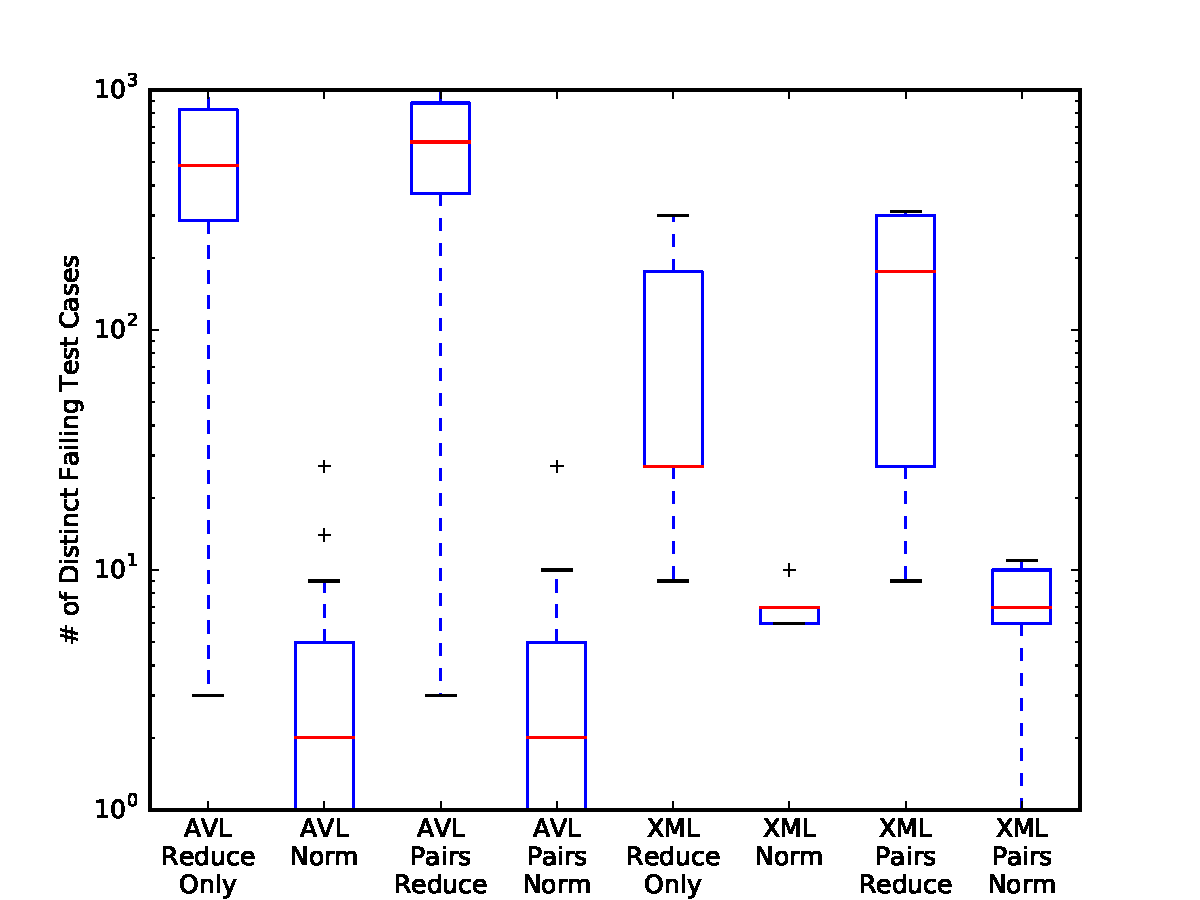
\includegraphics[width=\columnwidth]{length}
\caption{Effects of normalization on 82 AVL Tree mutants.}
\label{normeffect}
\end{figure}

Figure \ref{normeffect} shows the reduction in number of distinct
failing test cases produced by normalization (vs. reduction only) for
a set of 82 mutants \cite{mutant} of the AVLTree source code \cite{Hunter:2007}.  Of the 228 mutants
produced by MutPy \cite{mutpy}, only these produced at least 1 failure
in 1,000 test cases.  Using only delta-debugging-based reduction, the
mean number of distinct failures for each mutant (which is, by definition,
a single fault) was 498.4, with a median of 485.  Using normalization,
the mean was 3.1 distinct failures, with a median of just 2 failures.
For 38 of the 82 mutants, normalization produced only a single
representative failure.  For every mutant, normalization reduced the
number of distinct failures, and no mutant produced more than 27
distinct failures, after normalization.

The mean cost to reduce a
test case was 0.05 seconds, with a median of 0.03 seconds.  The mean
cost for normalization was 0.38 seconds, with a median of 0.1 seconds.
The minimum runtime for both algorithms was negligible (less than 1
millisecond), but the maximums were 1.3 seconds for reduction and 17.6
seconds for normalization.  Note that in all our results the cost of
normalization is given on an already-reduced test case, so the inputs
for normalization are smaller than those for reduction; however, this
is the expected use-case for normalization.  Comparing on equal-sized
tests would simply involve adding the costs for reduction to those for
normalization, as an additional step of normalization.  Finally, the
criticality of caching for normalizing large numbers of tests is
evident.  Out of 60,226 normalizations performed in our full AVLTree mutant
experiments, 59,972 (99.6\%) resulted in a cache hit (most of these
after a small number of normalization steps).  In fact, the total
number of rewrites performed during the experiments was only 145,780,
for an average of only 2.4 non-cache-hit rewrites of each test.  Note
that this is with the cache starting empty for each of the 82 mutants.

AVLTree mutants also provided a way to evaluate the danger of
normalization losing faults.  Faults can be lost when normalization
changes a test case failing due to one fault into a test case failing
due to a different fault, a problem known as ``slippage''
\cite{PLDI13}.  AVLTree provides a slippage challenge, as there are
very few API calls, and all calls take the same inputs, so test cases
for faults are likely to be very close to each other in the
combinatorial space.  To test the slippage rates for normalization, we
randomly selected 364 mutant pairs drawn from the 82 detectable
mutants, and produced higher-order-mutants for each of these by
applying both mutants to the source (using only mutants that modified
different source lines).  Of these, the set of reduced test cases
included at least one test capable of exposing each of the two faults
for only 238 pairs.  In almost all cases this was due to reduction
slippage, but in a few cases it was due to one fault completely
masking another: e.g., if {\tt insert} always fails, it is not
possible to produce a test case that exposes a fault in {\tt delete}
on a non-empty tree.

Out of these 238 mutant pairs, normalization produced test cases
exposing both faults for 80.7\% of pairs (19.3\% slippage at the
suite level).  Interestingly, in 4 cases
normalization took a set of reduced test cases not capable of exposing
both faults, and produced a smaller set of test cases that was capable
of detecting both faults.  Arguably this is ``slippage'' in that a test case not
capable of exposing fault F was modified to expose fault F (classic
slippage) but since the new test suite exposed both faults,
normalization actually restored fault detection.

Data on slippage is not extensive, in part because it is only detected if the original test
cases before reduction are stored and re-executed after bugs have been
fixed.  In our own previous work \cite{PLDI13}, slippage due to
reduction was extremely rare for some SUTs (GCC 4.3.0) and very common
for other SUTs (up to 23\% for Mozilla's JavaScript engine).  For our
own AVLTree example, the slippage rate for reduction is almost 30\%,
considerably worse than that for normalization.  As a simple mitigation, we propose
storing at least reduced test cases, and ideally the unreduced test
cases, as a slippage check when all faults detected by normalized test
cases are fixed.

The reduction in test cases produced by normalization for mutant pairs
was, as with single mutants, very large (Figure \ref{normeffect}).
For mutant pairs, the mean/median number of distinct failures was
554.4/607 for reduction alone, but only 2.8/2 for reduction +
normalization.  The runtime for normalization was essentially
unchanged from the single-mutant numbers given above.  For reduction
alone, using pairs increased the number of distinct failures, while
normalized failure counts decreased.  For 48.3\% (115 of 238) of
mutant pairs where reduction did not lose a fault, normalization
worked as well as possible --- it preserved both faults and produced only 1 or 2 test
cases\footnote{It is possible to detect both faults with a single test
  case, if that test case fails when \emph{either} fault is present.}.

\subsection{XML Parser}

We also examined how normalization combined with multiple faults for a
simple XML parser with about 260 lines of code \cite{myxml}, with one
real fault, triggered by the empty tag ({\tt <>})), and one
seeded fault triggered when adding two nodes with the same
name.  A comment in the code indicates the seeded fault is realistic.  Running 1,000 tests
produced 848 failing test cases.  Without normalization, it took only
37.45 seconds to execute and delta-debug all 1,000 tests.  The output was 717 distinct failing test
cases.  Normalization increased the runtime to 354.7 seconds, but
reduced the number of failures to just 5: 3 
for the original fault and 2 for the seeded fault.
%Generalization took < 5 seconds.


\subsection{TSTL}

As noted in Section \ref{freshgen}, TSTL is used to test TSTL's own
API interface (the TSTL compiler is about 1,600 LOC; a compiled SUT is
often 30KLOC or larger).  We only discovered one fault while testing
the latest version of TSTL, the cache-related problem shown in Figure \ref{fig:mislead}.
Generating and reducing 100 test cases for it required 1,090 seconds
and produced 90 failures.  Normalization and generalization
increased total runtime to 3,690 seconds, and produced just 2 failures.

\subsection{NumPy}

Our final two case studies provide little information on the ability
of normalization to reduce the number of failing tests; for these
SUTs, failure rates are low enough or test case reduction runtimes high
enough that each failure is dealt with one-by-one.  However,
normalization and generalization are also useful for understanding
individual test cases.

NumPy \cite{NumPy} is a widely used Python library that
supports large, multi-dimensional matrices and provides a huge library
of mathematical functions.  The SciPy library for scientific
computing builds on NumPy.  Developing tests for NumPy is challenging,
because none of the authors are experts in numeric computation, and
the specification of correct behavior is often somewhat subtle.  As a
simple example, consider the test case in Figure \ref{numpyorig},
normalized and generalized in Figure \ref{numpynormgen}.  Prior to
normalization, understanding why the test case leads to a violation of
self-equality for an array is difficult.  After
normalization, it is much clearer what is happening: 1) {\tt array0}
contains {\tt NaN} and 2) this is correct behavior (the array
\emph{should} contain {\tt NaN}).  The greater length and much larger
number of operations involved in the original reduced test case
obscures this critical point.  In NumPy, array equality does not hold
for objects containing {\tt NaN}, so the assertion must be modified.
As far as we know, normalization transforms all instances of this
fault into this canonical test case, but our data (for fewer than 30
failures) is insufficient to make a definite claim, as the failure rate
is slightly less than 3 failures/100,000 tests on average.

Other, more complex, failures have also made it clear that
normalization is useful for additional test case length reduction for
NumPy, and that generalization makes any surprising restrictions on
test values clear.  For NumPy tests, normalization takes much longer
than reduction, in part due to the expense of operations on large
arrays.  For almost all test cases, the average time to reduce tests
is about 4-5 seconds, and the time for normalization is between 712
and 774 seconds.  The average time to discover a failing test case,
for comparison, is just over 400 seconds.  Generalization takes
between 52 and 59 seconds in these cases.  The exception was a test
case of 45,206 steps (!)  leading to a memory exhaustion error and
crash.  This was reduced (over a period of nearly a day) to a test
case with 10 steps, which then normalized (in only 2 hours) to a test
case with 8 steps.  The normalized test case involved no operations other than array
initialization, array flattening, and array
addition.  The reduced test case required larger dimensions, array
multiplication, and array subtraction, as well.  This is the only case in
which we have seen normalization time lower than reduction time,
without assistance from the cache.

\begin{figure}
{\scriptsize
\begin{code}
 dim1 = 1 
 shape2 = (dim1, dim1, dim1) 
 array1 = np.ones(shape2) 
 array0 = array1 * array1 
 array1 = array1 + array1 
 array4 = array0 + array1 
 array0 = np.reshape(array4,shape2) 
 array3 = array1 * array4 
 array2 = np.ravel(array4) 
 array5 = array2 - array3 
 array4 = array5 * array2 
 array1 = np.unique(array0) 
 array5 = array5 * array3 
 array0 = array1 * array5 
 array5 = np.unique(array0) 
 array1 = array4 - array2 
 array2 = array0.flatten() 
 array0 = array5 + array5 
 array5 = array5 + array2 
 array2 = array0 * array2 
 np.copyto(array5,array2) 
 array2 = array2 * array5 
 array3 = array0 * array2 
 array0 = array3 - array1 
 array4 = array3 * array0 
 array1 = array5 + array4 
 array5 = array0 * array1 
 array0 = array5 - array1 
 array4 = array0 * array3 
 array3 = array4 * array0 
 array1 = array5 + array3 
 array0 = array2 + array1 
 array5 = array5 - array0 
 array5 = array3 * array5 
 array0 = array1 + array5 
 array2 = array3 - array0 
 array4 = array2 * array1 
 array3 = array4 * array2 
 array2 = array0 - array0 
 np.copyto(array1,array3) 
 array4 = array2.flatten() 
 array1 = array1 * array4
 assert (np.array\_equal(array1,array1))
\end{code}
}
\caption{Original ``failing'' test case for numpy (42 steps).}
\label{numpyorig}
\end{figure}

\begin{figure}
{\scriptsize
\begin{code}
dim0 = 1                            \textcolor{black!60}{\# STEP 0}
\textcolor{black!60}{\#  or dim0 = 10 }
shape0 = (dim0)                     \textcolor{black!60}{\# STEP 1}
\textcolor{black!60}{\#  or shape0 = (dim0, dim0) }
\textcolor{black!60}{\#  or shape0 = (dim0, dim0, dim0) }
array0 = np.ones(shape0)            \textcolor{black!60}{\# STEP 2}
array0 = array0 + array0            \textcolor{black!60}{\# STEP 3}
array0 = array0 + array0            \textcolor{black!60}{\# STEP 4}
\textcolor{black!60}{\#  or array0 = array0 * array0 }
array0 = array0 * array0            \textcolor{black!60}{\# STEP 5}
array0 = array0 * array0            \textcolor{black!60}{\# STEP 6}
array0 = array0 * array0            \textcolor{black!60}{\# STEP 7}
array0 = array0 * array0            \textcolor{black!60}{\# STEP 8}
array0 = array0 * array0            \textcolor{black!60}{\# STEP 9}
array0 = array0 * array0            \textcolor{black!60}{\# STEP 10}
array0 = array0 * array0            \textcolor{black!60}{\# STEP 11}
array0 = array0 * array0            \textcolor{black!60}{\# STEP 12}
array0 = array0 * array0            \textcolor{black!60}{\# STEP 13}
array0 = array0 - array0            \textcolor{black!60}{\# STEP 14}
assert (np.array\_equal(array0,array0))
\end{code}
}
\caption{Normalized and generalized test case for numpy (15 steps).}
\label{numpynormgen}
\end{figure}

\subsection{Esri ArcPy}

Esri is the single
largest Geographic Information System (GIS) software vendor, with about 40\%
of global market share.  Esri's ArcGIS tools are extremely widely
used for GIS analysis, in government, scientific research, commercial
enterprises, and education.  Automation is essential for complex GIS analysis and
data management, and Esri has long provided tools
for programming their GIS software systems.  One such tool
(Esri's newest) is a Python site-package, ArcPy \cite{ArcPy}.  ArcPy is a complex library,
with dozens of classes and hundreds of functions distributed over
a variety of of toolboxes.  Most of the code involved in ArcPy
functionality is the C++ source for ArcGIS itself (which is not
available) but the released Python interface code alone is over 50KLOC.

In order to improve the reliability of ArcPy, we are developing a
TSTL-based framework for testing ArcPy itself, as well as libraries
based on ArcPy.  The ArcPy TSTL is already more than twice as large as
the next-largest TSTL harness previously studied, even though it only
includes a small portion of ArcGIS functionality so far. The first
stage of testing has resulted in discovery of multiple faults in
ArcPy/ArcGIS, six of which not only cause incorrect behavior but cause
a crash that also ends testing.  It is critical to understand these
faults, the set of behaviors that trigger them, and modify the test
definition to avoid triggering these faults while imposing minimal limitations
on thorough testing for other faults.

There is no space in this paper to elaborate on the details of this
large test effort (which has introduced numerous additional features
and modes to TSTL), but normalization and generalization have been
very useful in this process.  Figures \ref{esriorig} and
\ref{esrinormgen} show one crash-inducing test case, after initial
delta-debugging (from over 2,000 test steps) (Figure \ref{esriorig})
and after normalization and generalization (Figure \ref{esrinormgen}).
In this setting normalization has contributed a significant amount of
additional reduction over delta-debugging.  For the crash fault shown
in this paper, normalization reduced the length from 19 steps to 11
steps.  For three other crashes, normalization reduced the test cases
from 18 to 14 steps, from 27 to 20 steps, and from 20 to 16 steps. One crash fault only reduced from 10 steps to 9 steps, but the
omission was informative.  The cost of normalization is high --- in
our runs, it has taken from 17,340 seconds up to 24,769 seconds.
However, in this setting even delta-debugging is extremely expensive
--- the cost of reduction alone has ranged from 7,930 seconds to 8,688
seconds.  Generalization has taken between 3,203 and
 11,149 seconds.  These high costs are due to the need to run
tests in a sandbox environment to avoid killing the Python testing
process, and the runtime of complex GIS analyses, with individual
actions sometimes requiring minutes to execute.
Even under these circumstances, reducing, normalizing, and
generalizing test cases has been a more effective use of human time than
trying to understand the faults without these aids.  For example, in
the test case shown in this paper, it was important to understand that
the SQL query and selection type are not essential, but using a
freshly created layer will not result in a crash: the problem appears
to be that ArcGIS (or ArcPy) does not invalidate layers built from a
feature class when that feature class is deleted\footnote{In this
  instance, a generalization (the fresh values generalization in
  particular) is informative even though it does not allow any
  generalization; knowing that it was attempted, but prevented the
  failure, is also valuable.}.  The original, non-normalized test case
makes this far less clear, as the use of {\tt CopyFeatures} and the
multiplicity of shapefiles involved disguises the essence of the
problem.

Normalization and generalization are also being used to prepare an
API-behavior regression suite for ArcPy.  One of the challenges of
using a large API like ArcPy is that behavior of the system can change
from version to version.  In some cases this is due to new faults, or
fixed faults, but in other cases there is an undocumented change,
especially for unusual input combinations.  In order to assist ArcPy
developers, we are preparing a test suite that covers as much as
possible of the Python source in the latest version of ArcPy, 10.3,
and records the values returned.  For future versions of ArcPy (or
older versions), a ``semantic diff'' with 10.3, based on these calls,
can be produced by running this suite.  The tests in the suite are
normalized and generalized to help users understand the set of
conditions behind an API usage's behavior.  This ``coverage
regression'' quick test \cite{icst2014} will also be
useful for understanding  the API, since the set of online examples of usage
from Esri is usually limited to a small set of parameter combinations.

\begin{figure}
{\scriptsize 
\begin{code}
shapefile2 = "C:\\arctmp\\new3.shp" 
shapefile1 = "C:\\arctmp\\new3.shp" 
featureclass2 = shapefile2 
featureclass0 = shapefile1 
shapefilelist2 = 
   glob.glob("C:\\Arctmp\\*.shp") 
fieldname0 = "newf3" 
shapefile1 = shapefilelist2 [0] 
featureclass1 = shapefile1 
arcpy.CopyFeatures\_management
   (featureclass1,featureclass2) 
op1 = ">" 
newlayer2 = "l2" 
val1 = "100" 
selectiontype2 = "SWITCH\_SELECTION" 
fieldname1 = "newf1" 
arcpy.MakeFeatureLayer\_management
   (featureclass0, newlayer2) 
arcpy.SelectLayerByAttribute\_management
   (newlayer2,selectiontype2,
   ' "'+fieldname0+'" '+op1+val1) 
op0 = ">" 
arcpy.Delete\_management(featureclass2) 
arcpy.SelectLayerByAttribute\_management
   (newlayer2,selectiontype2,
   ' "'+fieldname1+'" '+op0+val1) 
\end{code}
}
\caption{Original test case for ArcPy library (19 steps).}
\label{esriorig}
\end{figure}

\begin{figure}
{\scriptsize 
\begin{code}
shapefilelist0 = 
   glob.glob("C:\\Arctmp\\*.shp")        \textcolor{black!60}{\# STEP 0}
\textcolor{black!60}{\#[}
shapefile0 = shapefilelist0 [0]        \textcolor{black!60}{\# STEP 1}
newlayer0 = "l1"                       \textcolor{black!60}{\# STEP 2}
\textcolor{black!60}{\#  or newlayer0 = "l2" }
\textcolor{black!60}{\#  or newlayer0 = "l3" }
\textcolor{black!60}{\#  swaps with steps 3 4 5 6 7}
\textcolor{black!60}{\#] (steps in [] can be in any order)}
\textcolor{black!60}{\#[}
featureclass0 = shapefile0             \textcolor{black!60}{\# STEP 3}
\textcolor{black!60}{\#  swaps with step 2}
fieldname0 = "newf1"                   \textcolor{black!60}{\# STEP 4}
\textcolor{black!60}{\#  or fieldname0 = "newf2" }
\textcolor{black!60}{\#  or fieldname0 = "newf3" }
\textcolor{black!60}{\#  swaps with steps 2 8}
selectiontype0 = "SWITCH\_SELECTION"    \textcolor{black!60}{\# STEP 5}
\textcolor{black!60}{\#  or selectiontype0 = "NEW\_SELECTION" }
\textcolor{black!60}{\#  or selectiontype0 = "ADD\_TO\_SELECTION" }
\textcolor{black!60}{\#  or selectiontype0 = "REMOVE\_FROM\_SELECTION"}
\textcolor{black!60}{\#  or selectiontype0 = "SUBSET\_SELECTION"}
\textcolor{black!60}{\#  or selectiontype0 = "CLEAR\_SELECTION"   }
\textcolor{black!60}{\#  swaps with steps 2 8}
op0 = ">"                              \textcolor{black!60}{\# STEP 6}
\textcolor{black!60}{\#  or op0 = "<" }
\textcolor{black!60}{\#  swaps with steps 2 8}
val0 = "100"                           \textcolor{black!60}{\# STEP 7}
\textcolor{black!60}{\#  or val0 = "1000" }
\textcolor{black!60}{\#  swaps with steps 2 8}
\textcolor{black!60}{\#] (steps in [] can be in any order)}
arcpy.MakeFeatureLayer\_management
   (featureclass0, newlayer0)          \textcolor{black!60}{\# STEP 8}
\textcolor{black!60}{\#  swaps with steps 4 5 6 7}
arcpy.SelectLayerByAttribute\_management
   (newlayer0,selectiontype0,
   ' "'+fieldname0+'" '+op0+val0)      \textcolor{black!60}{\# STEP 9}
arcpy.Delete\_management(featureclass0) \textcolor{black!60}{\# STEP 10}
arcpy.SelectLayerByAttribute\_management
   (newlayer0,selectiontype0,
   ' "'+ fieldname0+'" '+op0+val0)     \textcolor{black!60}{\# STEP 11}
\end{code}
}
\caption{Normalized and generalized test case for ArcPy library
  (12 steps).}
\label{esrinormgen}
\end{figure}

\section{Related Work}

Chen et al. introduced the idea of slippage in the course of
describing efforts to automatically detect different faults in a large
set of failing test cases \cite{PLDI13}.  Hughes et
al. \cite{FindMoreBugs} proposed a modification of QuickCheck
to avoid re-producing known bugs that (in theory)
could mitigate the problem of slippage, but is not directly comparable
to our approach.  The approach of Hughes et al. requires
interpretation of test components (e.g. method calls), and analysis of
patterns, while our approaches are purely algorithmic, with no
additional requirements beyond those of delta debugging itself
\cite{DD}.  It is not clear how best to apply such an approach
 to cases such as {\tt jsfunfuzz} where each component is not a
method call but essentially an arbitrary string, without significant
user effort to define abstractions of components.

There are also approaches that sidestep slippage by initially
producing short test sequences (e.g. recent work by Mao et
al. \cite{Mao}).  However, for many generation algorithms
longer sequences are essential for good fault detection \cite{ASE08,LongBetter}.



\section{Conclusions}
\label{conclusion}

This paper reports on an end-user-driven automated testing effort for a Python
library used to automate Geographic Information System analysis and
data management.  The test system is based on the TSTL
\cite{NFM15,ISSTA15,tstl} domain-specific language for testing, which
enables a declarative style of test harness development, where the
focus is on defining the actions in valid tests, not determining
exactly how tests are generated.

The complexity, size, and some unusual features of
the SUT have driven some engineering decisions, enhancements to the
TSTL language, and new testing utilities.  This paper focuses on
presenting the experience of testing a large complex system, and (we
hope) demonstrates that a domain expert whose programming experience
consists almost entirely of using the Software Under Test can make use
of modern automated test generation methods to find faults in complex software systems.

%\IEEEtriggeratref{21}

%\bibliographystyle{IEEEtran}
% argument is your BibTeX string definitions and bibliography database(s)

%\def\IEEEbibitemsep{0.6pt plus 0.9pt}

\bibliographystyle{abbrv}
\bibliography{bibliography}

\end{document}
